\documentclass[12pt, english, letterpaper]{kuthesis}
\usepackage{mathptmx}
\renewcommand{\sfdefault}{lmss}
\renewcommand{\ttdefault}{lmtt}
\usepackage[T1]{fontenc}
\usepackage[utf8]{inputenc}
\usepackage{geometry}
\geometry{verbose,tmargin=1in,bmargin=1in,lmargin=1in,rmargin=1in}
\setcounter{secnumdepth}{3}
\setcounter{tocdepth}{3}
\usepackage{color}
\usepackage{babel}
\usepackage{url}
\usepackage{graphicx}
\usepackage{setspace}
\usepackage{esint}
\usepackage[authoryear]{natbib}
\doublespacing
\usepackage[unicode=true,
 bookmarks=true,bookmarksnumbered=false,bookmarksopen=false,
 breaklinks=true,pdfborder={0 0 0},pdfborderstyle={},backref=false,colorlinks=true]
 {hyperref}
\hypersetup{pdftitle={Promise Land},
 pdfauthor={Andrei Elliott},
 pdfsubject={Javascript-style Promises with Strong Typing},
 urlcolor={black},citecolor={black},allcolors={black}}

\usepackage{relsize}
\usepackage{fancyvrb}
\usepackage[nameinlink, noabbrev]{cleveref}
\usepackage{tikz}


\usetikzlibrary{calc, matrix, positioning}
\tikzset{ gap/.style = {preaction={draw, line width=2pt, white}} }


\newcommand{\lit}[1]{\textbf{\texttt{#1}}}

\DefineVerbatimEnvironment{code}{Verbatim}{xleftmargin=2em,samepage=true,fontseries=b}
%\newenvironment{code}{\Verbatim}{\endVerbatim}
\interfootnotelinepenalty=8000

\title{Promise Land\\
\smaller Proving Correctness with Strongly Typed Javascript-Style Promises}
\author{Andrei Elliott}

\priorcreds{}

\dept{Electrical Engineering and Computer Science}
\degreetitle{Master of Science}
\papertype{Project Report}

\committee {Matt Moore}	{Perry Alexander}	{Drew Davidson}	{}	{}	{}	{}
\role      {Chair}	{}	{}	{}	{}	{}	{}



\makeatletter
\@printd@testrue
\datedefended{Friday May 6, 2022}
\dateapproved{Friday May 6, 2022}
\makeatother

\begin{document}

\begin{romanpages}
  \maketitle
  \begin{abstractlong}
    Code that can run asynchronously is important in a wide variety of situations, from user interfaces to communication over networks, to the use of concurrency for performance gains.  One widely-used method of specifying asynchronous control flow is the \textsf{Promise} model as used in Javascript.  \textsf{Promises} are powerful, but can be confusing and hard to debug.  This problem is exacerbated by Javascript’s permissive type system, where erroneous code is likely to fail silently, with values being implicitly coerced into unexpected types at runtime.

The work presented here implements Javascript-style \textsf{Promises} in Haskell, translating the model to a strongly typed framework where we can use the type system to rule out some classes of bugs.  Common errors --- such as failure to call one of the callbacks of an executor, which would, in Javascript, leave the \textsf{Promise} in an eternally-\emph{pending} deadlock state --- can be detected for free by the type system at compile time and corrected without even needing to run the code.

Along the way, we demonstrate that \textsf{Promises} form a monad, providing a monad instance that allows code using \textsf{Promises} to be written using Haskell’s \lit{do} notation.
  \end{abstractlong}
%  \tableofcontents {}
\end{romanpages}

\chapter*{Introduction}
One widely-used model of concurrency is Javascript's \textsf{Promises}, initially proposed in \cite{friedman}.  A promise works in some ways like a lazy value, in that it will at some point contain the result of a computation, but does not stop flow of control in the current thread to compute that value.  Unlike a value with lazy semantics, a promise can immediately begin computation in a separate thread as opposed to waiting for the result to be requested by some other computation.

\textsf{Promises} are composable: using \lit{then} and \lit{catch}, we can chain a promise onto the end of a different one creating a new promise that continues computation after the first has succeeded or failed respectively.  Additionally, \textsf{Promises} can be combined in parallel, with a variety of distinct semantics such as waiting for the first success or for the first completion irrespective of success or failure.

\cite{madsen} notes that programmers often make mistakes when writing code involving \textsf{Promises} and Javascript provides no static checks to detect these errors.  By implementing the \textsf{Promise} interface in Haskell, we create a \textsf{Promise} library where the success and failure types associated with a given \lit{Promise} value are tracked in the type system so that mismatches can be detected by the type checker at compile time rather than causing errors at run time.  By carefully choosing the type of the function that creates new \lit{Promise} values, we can cause the type checker to also reject programs containing bugs of the type \cite{madsen} classified as ``Dead Promise''.

Additionally, we provide typeclass instances, including \lit{Monad} for our \lit{Promise} type, allowing it to be easily used with existing Haskell code.

In the following section, we discuss the basics of Haskell and of the \textsf{Promise} model.  Next, we walk through the implementation of our \textsf{Promise} library in detail.  Finally, we discuss what guarantees we gain by using our strongly typed system; which classes of errors would be caught by it and how common they are.  Appendix A contains our complete source code.
\chapter*{Background}
\section*{Haskell}
We will refer to types in Haskell syntax.  We may say that a value \lit v has type \lit T and write this as \lit{v ::\ T}.  Specific types are capitalized, e.g. \lit{3 ::\ Integer}, while type variables are written in lowercase and are usually a single character.  Some types are paramterized by other types.  For instance, Haskell lists are linked lists of values that share a type.  A list containing values of type \lit T will itself have the type \lit{[T]}, that is, list-of-T.  Perhaps the most common variety of parameterized type to see in Haskell type signatures is the function, written with an ASCII arrow (\lit{->}).  Functions are parameterized by the types of both their input and output; a function that counts the lengths of \lit{String}s could have the type \lit{String -> Integer}.  The syntax for calling functions is simple juxtoposition: the expression \lit{f x} means the function \lit f applied to \lit x.  Functions with more than one argument are \emph{curried}, for example a two argument function that takes an \lit A and a \lit B as input to produce a \lit C is written with the type \lit{A -> B -> C}, i.e.,  a function that accepts an \lit A and returns another function that accepts a \lit B and returns a \lit C\footnote{\lit{->} associates to the right to facilitate writing curried functions without parentheses}.

Generalized Algebraic Data Type, or GADT, syntax allows us to specify our own types and give the name and type for each \emph{constructor} function that can create a value of that type.  We will write one defining the type \lit{Promise f p} which will represent a \lit{Promise} that yields a result with the type \lit p if it succeeds or one of type \lit f on failure.

We will discuss what types various objects should have and will, at times, need a convention to refer to a parameterized type when we haven't yet decided what the parameter will be.  In these cases, \lit ? is a metavariable representing some concrete type yet to be decided, rather than real syntax.  \lit{Integer -> ?\ -> ?} means a two-argument function accepting an \lit{Integer} and some type we will decide later that returns another value of the same type.  This is distinct from \lit{Integer -> a -> a} using type variables because the latter is a function accepting an \lit{Integer} and any value whatsoever, returning a value of the same type as the input.

Values in Haskell are referentially transparent, meaning that if an expression evaluates to a value, it can be replaced by that value with no change to the program's semantics.  This makes it easier to reason about and prove properties of programs, but comes with a few challenges.  For instance, a print statement should not be replaced with a value without executing.  Haskell solves this problem with the \lit{IO} monad.  A value of type \lit{IO T} can be thought of as an action that will result in a value of type \lit T, but may also have side effects.  An action that is performed solely for its side effects and has no useful result value is conventionally given the type \lit{IO ()}.  The type \lit{()}, pronounced ``unit'' is the type of tuples holding no objects.  There is only one value of this type, also written \lit{()}.  The contents of \lit{IO} values can only be interacted with through the interface of the monad typeclass.  In particular, there is no way to convert an \lit{IO T} into a \lit{T}; you cannot get a value out of \lit{IO}.  The \emph{do notation} provides a friendly, imperative-looking syntax for interacting with monadic values.  In code like the following, the expression \lit{ioThing} returns a value wrapped in a monad.
\begin{code}
 do
  x <- ioThing
  . . .
\end{code}
The arrow (\lit{<-}) binds the value so wrapped to the variable \lit x and in the region of the code marked by elipses (\lit{\(\dots\)}), \lit x can be treated as a normal non-monadic value.  However, at the end of the block, the final expression must be re-encapsulated into the monad.  The simplest way to do this is the function \lit{return}.  \lit{return x} simply puts the value \lit x into a default context in the monad.

In order to implement \textsf{Promises}, we need asynchronous action.  To accomplish this in Haskell, we will use \lit{forkIO} and \lit{MVar}s.  The function \lit{forkIO ::\ IO () -> IO ThreadId} accepts an \lit{IO ()} action and runs it in a separate thread.  In order to communicate between threads, we use \lit{MVar}s.  A value of type \lit{MVar T} is a thread-safe place to store up to one value of type \lit T.  We interact with \lit{MVar}s with three functions:
\begin{itemize}
\item \lit{newEmptyMVar ::\ IO (MVar a)} \\
  Creates an \lit{MVar} with no
  contents.  The type variable \lit a will usually be inferred by what
  type we try to add later.
\item \lit{putMVar ::\ MVar a -> a -> IO ()}\\
  Accepts a value of type \lit a and stores it in the \lit{MVar}.  If
  the \lit{MVar} already contains a value, the thread running
  \lit{putMVar} will block until the \lit{MVar} is empty.
\item \lit{takeMVar ::\ MVar a -> IO a} \\
  Reads an \lit{IO a} from the
  \lit{MVar}, leaving it empty, and will block, if necessary, until
  there is a value in the \lit{MVar} to be read before doing so.
\end{itemize}
\section*{Promises}

A \textsf{Promise} represents a unit of computation to be performed asynchronously.  When one is created, the work to be done is specified as a function to be executed.  This computation occurs without interrupting the control flow at the site that created the \textsf{Promise}.  Since the work represented by a \textsf{Promise} may not have been completed yet, any values that result can't be used directly.  Instead, we can \emph{chain} \textsf{Promises} by using \lit{then} to schedule code that depends on the result, creating a new \textsf{Promise} representing the initial work followed by the additional code.  A \textsf{Promise} that succeeds will execute code chained after it with \lit{then}; one that fails will execute any that was chained after it with \lit{catch}.  In either case, this will happen one the initial \textsf{Promise} has finished running and \lit{then} or \lit{catch} has been called, regardless of which order those two events happen in.

\textsf{Promises} can be in one of three states: \emph{pending}, \emph{fulfilled}, or \emph{rejected}.  The \emph{pending} state represents a \textsf{Promise} that is still running.  A \textsf{Promise} that has completed with a success value is in the \emph{fulfilled} state; the process of moving from \emph{pending} to \emph{fulfilled} is referred to as the \textsf{Promise} \emph{resolving}.  The state for a failed \textsf{Promise} is called \emph{rejected} and to \emph{reject} a \textsf{Promise} is to move it from the \emph{pending} state to the \emph{rejected} state.  For a \textsf{Promise} to \emph{settle}, it moves from \emph{pending} to either \emph{fulfilled} or \emph{rejected}.  \Cref{fig:states} summarizes this terminology.

\begin{figure}
\begin{center} 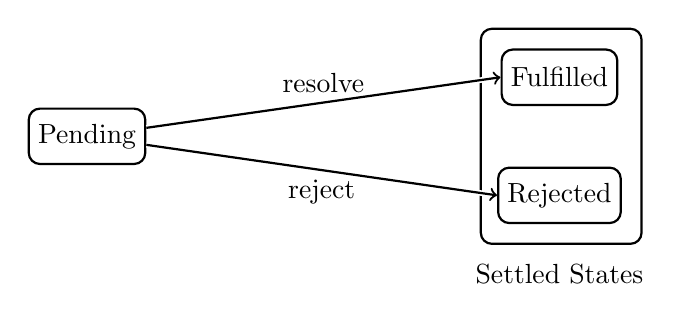
\begin{tikzpicture}
  \path (0,0) node[draw, thick, rounded corners, minimum height=2em, minimum width=4em] (pend) {Pending}
      ++(6,0.75) node[draw, thick, rounded corners, minimum height=2em, minimum width=4em] (ful) {Fulfilled}
      ++(0,-1.5) node[draw, thick, rounded corners, minimum height=2em, minimum width=4em] (rej) {Rejected}
      ++(0,-1) node {Settled States};

  \draw[rounded corners, thick] ($(ful.north west)+(-0.25,0.25)$) rectangle ($(rej.south east)+(0.25,-0.25)$);
  \draw[thick] (pend) edge[gap,->] node[above] {resolve} (ful.west) (pend) edge[gap,->] node[below] {reject} (rej.west);
\end{tikzpicture} \end{center}
\caption{States and Transitions.}
\label{fig:states}
\end{figure}

\chapter*{Haskell Implementation}

\section*{Making a Promise}
Javascript's \lit{Promise()} constructor builds a new promise object from an `executor' function.  The executor accepts two callback functions: resolutionFunc and rejectionFunc, one to call in the case of successful resolution and the other for failure.  The executor will, on a success or failure, call \lit{resolutionFunc} or \lit{rejectionFunc}, respectively, passing in the value of or reason for the success or failure.  Let's assume we want a promise with type \lit{Promise f p}, i.e. one where success results in a value of type \lit p and failure gives a reason with type \lit f.  To build such a \lit{Promise}, \lit{resolutionFunc} will need to accept a value of type \lit p.  Since calling \lit{resolutionFunc} will settle the promise and therefore have effects elsewhere in the promise chain, its return type will have to be something wrapped in \lit{IO}, so we know \lit{resolutionFunc ::\ p -> IO ?}.  Similarly, \lit{rejectionFunc} must accept a \lit f, and calling it will also settle the promise, so \lit{rejectionFunc ::\ f -> IO ?}.  The executor function should accept \lit{resolutionFunc} and \lit{rejectionFunc} as parameters and is expected to end by calling exactly one of them, so we will expect it to have a proper tail call to one of the parameters.  This means its return type matches that of \lit{resolutionFunc} and \lit{rejectionFunc}, i.e.
\begin{code}
executor :: (p -> IO ?) -> (f -> IO ?) -> IO ?
\end{code}
  For now, let's use \lit{()} as \lit ?, so that the callbacks have a return type of \lit{IO ()}, the conventional Haskell type for \lit{IO} actions that only have an effect (here, setting the Promise from \lit{Pending} state to one of the settled states) instead of containing a useful value.  Our function for building a \lit{Promise} object needs to accept a function with the type of \lit{executor} and give back a \lit{Promise} value, which must be contained in \lit{IO} because it has the side effect of running the \lit{executor} in another thread.  It thus has the type:
\begin{code}[xleftmargin=0em]
newPromise :: ((p -> IO ()) -> (f -> IO ()) -> IO ()) -> IO (Promise f p)
\end{code}
We can represent a \lit{Promise f p} by an \lit{MVar (Either f p)}.  Once the computation for the \lit{Promise} is complete, it can be written to with an \lit{Either f p} value, i.e. \lit{Left reason} for a failure or \lit{Right result} in the case of success.  \lit{newPromise} will also need to fork a thread that will run the executor and set up communication so that the final \lit{Promise} object will be updated with the results once they are available.  In total, we need to: create an \lit{MVar} which we'll call \lit{state}, then fork a thread that calls the executor, passing it callback functions that write the results to \lit{state}, and finally, return \lit{state} as a \lit{Promise} value.
\begin{code}
newPromise :: ((p -> IO ()) -> (f -> IO ()) -> IO ())
              -> IO (Promise f p)
newPromise k = do
  state <- newEmptyMVar
  forkIO $ k (putMVar state . Right) (putMVar state . Left)
  return (Pending state)
\end{code}
% $
Since the constructor here is used to create \textsf{Promises} that are in the \emph{pending} state, we'll call it \lit{Pending}.  We could, in principle, use this same constructor to build \lit{Promise} values that we know have already succeeded or failed.  To get a promise that always succeeds with a value of \lit s, say, we could simply call \lit{newPromise} with an executor that immediately calls \lit{successFunc}, like so:
\begin{code}
newPromise (\ succeed fail -> succeed s)
\end{code}
This is inefficient, though, because it spawns an entire new thread in order to do absolutely nothing with it.  Instead, it is easy enough to define a constructor that marks a value as known to be the result of a sucessful computation (and a parallel one declaring a value to be the known reason for a failed computation).  These correspond to the promise being in the state \emph{fulfilled} or \emph{rejected}, repectively, so we will uses those terms as the names the constructors.  At this point, the \lit{Promise} type has the following form, in GADT syntax:
\begin{code}
data Promise :: * -> * -> * where
  Pending :: MVar (Either f p) -> Promise f p
  Fulfilled :: p -> Promise f p
  Rejected :: f -> Promise f p
\end{code}
What happens if we use a type other than \lit{()} in place of \lit ? in the \lit{newPromise} function?  Say we use the type $\tau$.  The executor function passed in must evaluate to an \lit{IO $\tau$}.  If the executor ends in a call to either \lit{resolutionFunc} or \lit{rejectionFunc}, it will work exactly the same no matter what type $\tau$ represents.  When using \lit{newPromise}, we can use the same code we did before in the \lit{$\tau = $()} case.  When \lit{ executor} doesn't contain a tail-call to one of its argument functions, the type $\tau$ matters for whether \lit{newPromise executor} typechecks; in particular, it will be accepted if and only if whatever \lit{executor} is doing \emph{other than} calling one of its callbacks yields the result type \lit{IO $\tau$}. In this situation, the resulting \lit{Promise} will never settle and any further actions chained to it will never run.  Unintentionally causing this state of affairs in that manner was the cause of multiple errors in the case study from \cite{madsen}. If we were to select a type $\tau$ that doesn't appear as the result of normal code, we could have Haskell's type system automatically detect this entire class of bugs at compile time.  One option would be Haskell's \lit{Void} type, which has no constructors.  But there may be cases where we legitimately need a \lit{Promise} that will never resolve (for example, the Javascript standard specifes that the result of calling \lit{Promise.race()} on the empty list results in such a \textsf{Promise}).  Furthermore, we need to create a value of type \lit{IO $\tau$} when implementing \lit{newPromise}.  Therefore, instead of using \lit{Void}, we create a new type unused anywhere else.  We name this type \lit{Token} because its only value is that you need one to write an \lit{executor} function.
We can provide a value \lit{hangForever ::\ IO Token} representing the behavior of remaining in the \emph{pending} state indefinitely and never resolving.  This allows the user who wants that behavior to specify it while making it unlikely to occur by accident.
\begin{code}
data Token = MkToken

hangForever :: IO Token
hangForever = return MkToken
\end{code}
Using \lit{Token}, our \lit{newPromise} code now needs to use \lit{fmap} to convert \lit{resolutionFunc} and \lit{rejectionFunc} to the correct types and again to convert the argument to \lit{forkIO} from \lit{IO Token} to \lit{IO ()}:
\begin{code}
newPromise :: ((p -> IO Token) -> (f -> IO Token) -> IO Token)
              -> IO (Promise f p)
newPromise k = do
  state <- newEmptyMVar
  forkIO $ fmap (const ()) $ k (fmap (const MkToken)
                                     . putMVar state . Right)
                               (fmap (const MkToken)
                                     . putMVar state . Left)
  return (Pending state)
\end{code}

\section*{What Then?}
Now that we can create \lit{Promise} values, the next step is to allow them to chain together.  Javascript's \lit{Promise.then()} is used to set a handler function to run after a promise completes.  Specifically, \lit{p1.then(f)} results in a new promise that will wait for the \lit{Promise} \lit{p1} to complete.  If \lit{p1} succeeds and resolves to a value \lit v, it will then call \lit{f(v)}.  The result of running the callback should be another \lit{Promise}, \lit{p2}; when it settles, the new \lit{Promise} will also settle, to the same state and value\footnote{Javascript also allows the callback to return a non-\lit{Promise} value, in which case \lit{p1.then(f)} resolves to that value as soon as it's computed.  We won't implement this functionality directly
as allowing differing argument types would not work in Haskell's type system unless we made separate \lit{then} functions for the two variants.  However, we can get to the same result by enclosing the value we would like to return in an always-successful \lit{Promise}.  Once we define a monad instance for \lit{Promise f}, we can even do so by writing \lit{return v} (where \lit{v} is the value for the final promise to resolve to), which should look familiar to anyone used to the Javascript syntax!}.
In our system in Haskell, \lit{pThen} accepts \lit{pr}, a \lit{Promise f p} along with a callback that expects a value of type \lit p, the type contained in a sucessful \lit{Promise f p}.  \lit{pThen} will return a \lit{Promise} (in \lit{IO} because we need to be able to read the \lit{state} \lit{MVar}), which must have the same failure type as \lit{pr} because if \lit{pr} is Rejected, the result will be as well, with the same value.  The result type can have a different sucess type, though, so it's overall type is \lit{IO (Promise f p')}.  The callback returns a new \lit{Promise} in IO, which must match \lit{pThen}'s return type, so in total
\begin{code}
pThen :: Promise f p
        -> (p -> IO (Promise f p'))
        -> IO (Promise f p')
pThen (Pending state) k = do
  result <- readMVar state
  case result of
    Left x -> return $ reject x
    Right x -> k x
pThen (Fulfilled x) k = k x
pThen (Rejected x) k = return $ reject x
\end{code}
      
Note that the type signature for \lit{pThen} looks extremely similar to the type \lit{(>>=)} would have if it were to be specialized to \lit{Promise f}.
\begin{code}
(>>=) :: Promise f a -> (a -> Promise f b) -> Promise f b
\end{code}
The difference is that \lit{pThen} is entangled in the \lit{IO} monad.

 \lit{Promise.catch()} works the same way as \lit{.then()} except that the handler is set to run only if and when the \lit{Promise} it is being chained to fails, rather then when it succeeds.  Our translation to Haskell, \lit{pCatch}, is very much like \lit{pThen} except that the code for a failed promise and a successful one have swapped places.  Its type is
 \begin{code}
pCatch :: Promise f p
        -> (f -> IO (Promise f' p))
        -> IO (Promise f' p)
\end{code}
which is the same as that for \lit{pThen} except that it operates on the type \lit f, the type of failure cases, instead of \lit p, the type of success cases.
\begin{code}
pCatch (Pending state) k = do
  result <- readMVar state
  case result of
    Left x -> k x
    Right x -> return $ resolve x
pCatch (Fulfilled x) k = return $ resolve x
pCatch (Rejected x) k = k x
\end{code}
\lit{pCatch} is dual to \lit{pThen} in that it is identical to a \lit{pThen} that operates on \lit{Promise}s with reversed semantics for which type argument represents success and which represents failure.

\lit{pThen} and \lit{pCatch} both share the same central function of waiting, if necessary, for a \lit{Promise} to settle, then branching on whether the result was a success or a failure.  We can generalize this behavior by writing a single function that accepts arguments specifying what to do in either case.  The action \lit{yes}, to do in the case of success can depend on the particular value the promise resolved with, so it should be a function accepting values of type \lit p.  The overall result of \lit{runPromise} must be contained in the IO monad because we can only compute it with the side effect of waiting for the \lit{Promise} to settle.  The return type of \lit{yes} should match that of runPromise, so \lit{yes ::\ p -> IO ?}.  There are no other restrictions on ?, so we can choose \lit{yes ::\ p -> IO a}. The function \lit{no} must also match return types so \lit{no ::\ f -> IO a}.

\begin{code}
runPromise :: (p -> IO a) -> (f -> IO a) -> Promise f p -> IO a
runPromise yes no (Pending state) = do
  result <- readMVar state
  case result of
    Left x -> no x
    Right x -> yes x
runPromise yes _ (Fulfilled x) = yes x
runPromise _ no (Rejected x) = no x
\end{code}
Now we can avoid code duplication by rewriting \lit{pThen} and \lit{pCatch} in terms of \lit{runPromise}, as follows:

\begin{code}
pThen p k = runPromise k (return . reject) p

pCatch p k = runPromise (return . resolve) k p  
\end{code}
\lit{runPromise} has the semantics of the two argument form of Javascript's \lit{Promise.then()}, adding to the chain in both the success case and the failure case. 

Similarly to Javascript's \lit{Promise.finally()}, the function \lit{pFinally} runs a \lit{Promise}, then chains to the \lit{Promise} passed as its argument regardless of how the former settles.  We can implement it by generating the function \lit{const k} which ignores its input and always returns \lit{k}, the \lit{Promise} to chain to.  We then pass this constant function as both the \lit{yes} and \lit{no} arguments to \lit{runPromise}.

\begin{code}
pFinally :: Promise f p
         -> IO (Promise f' p')
         -> IO (Promise f' p')
pFinally p k = runPromise (const k) (const k) p
\end{code}

It is sometimes helpful to run a \lit{Promise} to completion to yield a non-\lit{Promise} value storing the results.  A function to do so has the type \lit{Promise f p -> IO (Either f p)}.  The result must be in \lit{IO} and is either a \lit{Left f} representing failure with the given reason or a \lit{Right p} representing success with the given value.  Implementing such a helper function is as simple as calling \lit{runPromise} and passing in a \lit{yes} that wraps its input in \lit{Right} and \lit{IO} and a \lit{no} that wraps in \lit{Left} and \lit{IO}.  We call this function \lit{await} in analogy to the \emph{await} keyword in Javascript.  Similarities include that it converts from a \lit{Promise} to a non-\lit{Promise} value by waiting for it to complete and that it can only be used inside the appropriate context; either the \lit{IO} monad or an \emph{async} function, as appropriate.

\section*{Instances}
We noted earlier that \lit{pThen} had a form reminiscent of a monadic bind operation; it is now time to demonstrate the connection more directly by writing a Monad instance for \lit{Promises}.  This will, among other things, allow us to use \lit{do} notation with code employing \lit{Promise}s.  The \lit{Monad} typeclass operates on types of kind \lit{* -> *}, i.e. type ``containers'' that are parameterized by exactly one other type.  But \lit{Promise} takes two type parameters, having kind {* -> * -> *}.  We can fix this mismatch by defining an instance for the partially applied type \lit{Promise f} that has already taken one type parameter.  Because \lit f is fixed in the instance, a given invocation of a function from one of our instances will need to keep the type of the failure value constant, even if it changes the type of the success value.\footnote{This is the reason the failure type is specified before the success type in \lit{Promise f p}: it is more straightforward to write instances where the first parameter is held constant and being able to change the success type with \lit{fmap} is more useful.}
To define a Monad instance for \lit{Promise f}, we begin with \lit{Functor} and \lit{Applicative} instances.  For \lit{Functor (Promise f)}, we must define \lit{fmap} with type \lit{(a -> b) -> Promise f a -> Promise f b}.  \lit{fmap} must accept a function, \lit g, and a \lit{Promise}, \lit{pr}, as input and apply the \lit g to the success value of \lit{pr} if there is such a value, to yield a new \lit{Promise} (\lit{fmap} will have no effect on a \lit{Promise} that fails; we wouldn't be able to apply \lit g to the failure value since it has the wrong type).  It is simple enough to run \lit{pr} and then either apply \lit g to the result on a success or not on a failure, like so:
\begin{code}
  fmap' :: (a - > b) -> Promise f a -> IO (Promise f b)
  fmap' g pr = runPromise (return . resolve . g) (return . reject) pr
\end{code}
But we have a problem: computing \lit{fmap'} has a side effect - it waits until \lit{pr} has settled.  This side effect shows up in the type as we can see that \lit{fmap'} generates an \lit{IO (Promise f b)} instead of a \lit{Promise f b}.  When declaring a \lit{Functor} instance, the type of \lit{fmap} is specified exactly.  \lit{fmap'} isn't good enough  - \lit{Functor}s can be mapped over anywhere, not just inside the IO monad.  What we can do instead is store \lit g, so we can wait to apply it until we \emph{are} instructed to run \lit{pr}.  We can store \lit g by defining another constructor for \lit{Promise f p}.  We now know that there is another way to make a \lit{Promise} object: take an existing \lit{Promise} and store along with it a function to map over it.  We add a new line to the \lit{Promise} GADT, which now reads:
\begin{code}
data Promise :: * -> * -> * where
    Pending :: MVar (Either f p) -> Promise f p
    Fulfilled :: p -> Promise f p
    Rejected :: f -> Promise f p
    PromiseMap :: (a -> b) -> Promise f a -> Promise f b
\end{code}

At this point declaring the instance is as simple as telling Haskell to convert \lit{fmap} to our \lit{PromiseMap} constructor:
\begin{code}
instance Functor (Promise f) where
    fmap g pr = PromiseMap g pr
\end{code}
If that seemed too easy, that's because it was; we still need something like \lit{fmap'} to actually apply \lit g when it needs to be applied.  Our definition for \lit{runPromise} needs to say what to do when we try to run a \lit{PromiseMap}.  For this case, we can pattern match to \lit{runPromise yes no (PromiseMap g pr)}.  Unlike when defining \lit{fmap}, at this point, we are returning an \lit{IO Promise} so we can wait for the contained promise \lit{pr} to settle and decide whether or not to apply \lit g.  We can make a recursive call to \lit{runPromise} on \lit{pr}; we know this will terminate because \lit{pr} is structurally smaller than \lit{PromiseMap g pr} \footnote{for this to fail to terminate, we would need to be trying to run a \lit{Promise} with an infinite number of functions mapped over it}.  The \lit{no} function is unchanged since mapping over a failed \lit{Promise} has no effect, but in the case of a successful one, we need to call \lit g before we give the result to \lit{yes}.  This means the success function for the recursive call will be \lit{yes . g}, the composition of \lit{yes} and \lit g, that applies \lit g, then gives the result directly to \lit{yes}.
\begin{code}
runPromise yes no (PromiseMap g pr) = runPromise (yes . g) no pr
\end{code}

To define the Applicative instance \lit{Applicative (Promise f)}, we need to be able to put an arbitrary value into a \lit{Promise f} and to map a function that is itself the result of a \lit{Promise f} over the (successful) result of another \lit{Promise f}.  The first function we must provide is \lit{pure ::\ a -> Promise f a}.  \lit{pure} should put its argument into the context of a \lit{Promise} `containing' nothing else, which is precisely what \lit{resolve} does.  The other function to define for the Applicative instance is \lit{(<*>) ::\ Promise f (a -> b) -> Promise f a -> Promise f b}, which is like \lit{fmap} except that the function is also inside a \lit{Promise}.  Directly running the \lit{Promises} to get their results to combine can't happen outside \lit{IO}, so we will again need to encode the map into a new constructor for \lit{Promise} and unpack it in \lit{runPromise} to avoid the extraneous \lit{IO} in the type.  Rather than encoding \lit{(<*>)} directly, we can instead use the equivalent \lit{liftA2} construction that maps a two-argument function over two instances of the applicative. Specialized to \lit{Applicative (Promise f)}, \lit {liftA2} has the type \lit{(a -> b -> c) -> Promise f a -> Promise f c -> Promise f c}.  Given such a function, we can implement \lit{(<*>)} as \lit{f <*> x = liftA2 (\$) f x}, where \lit{(\$)} is the application function that accepts a function and an argument and applies one to the other.  Our new constructor is called \lit{PromiseMap2} because it maps over two arguments, and we add it to the GADT for \lit{Promise}:
\begin{code}
  PromiseMap2 ::  (a -> b -> c) -> Promise f a -> Promise f b -> Promise f c
\end{code}
and we define the instance as follows:
\begin{code}
instance Applicative (Promise f) where
  pure x = resolve x
  f <*> x = PromiseMap2 ($) f x
\end{code}
% $
The new case to \lit{runPromise} for mapping a function \lit g across two \lit{Promise}s creates a \lit{Promise} chain that waits for both arguments to resolve, then yields the value of \lit g applied to the results.
\begin{code}
runPromise yes no (PromiseMap2 g prA prB) = do
  pr' <- pThen prA $ \a ->
    pThen prB $ \b -> return $ resolve $ g a b
  runPromise yes no pr'
\end{code}
Note that, while using a \lit{do} block here may look circular since we haven't yet defined the monad instance for \lit{Promise f}, this \lit{do} is in the \lit{IO} monad rather than \lit{Promise}.

The instance for \lit{Monad (Promise f)} requires \lit{return ::\ a -> Promise f a} that puts a value into a neutral context; this can be the same as \lit{pure} from \lit{Applicative}.  The other function required to declare a Monad instance is \lit{(>>=)} (pronounced ``bind'') and, when specialized to \lit{Promise f}, has the type \lit{Promise f a -> (a -> Promise f b) -> Promise f b}.  That is, it accepts a \lit{Promise}, \lit p, as well as a function, \lit k, that converts from a plain value of the type of a sucessful result from \lit p.  Then, \lit{(>>=)} applies \lit k to \lit p as though \lit p were a plain value instead of a \lit{Promise}.  The type of \lit{(>>=)} is exactly that of \lit{pThen} except that it references unadorned \lit{Promise}s in the places where \lit{pThen} had \lit{IO Promise}s.  As will be familiar by now, we must add a new \lit{Promise} constructor so we can delay execution until \lit{runPromise}.  In this case, we can add
  \begin{code}
    PromiseJoin :: Promise f (Promise f a) -> Promise f a
  \end{code}
  which collapses a two-layer \lit{Promise} into a single layer.  Join is an equivalent characterization to \lit{(>>=)} as we can write
  \begin{code}
    p >>= k = PromiseJoin (fmap k p)
  \end{code}
  using \lit{fmap} to apply \lit k to \lit p before returning to a single layer of \lit{Promise} with \lit{join}.
  
  To implement \lit{pJoin}, we need to squash a double-decker \lit{Promise}, \lit{pp ::\ Promise f (Promise f a)}, down to a single layer.  We can do this with \lit{pThen}.  Normally, \lit{pThen} expects the function argument, \lit k, to be a function that adds a layer of \lit{Promise}ness to the input (as well as an IO wrapper): after all, it has the type \lit{p -> IO (Promise f p')}.  But what if we instead \emph{only} wrap \lit k's input in \lit{IO}?  Here \lit{k x = return x}, with the type \lit{b -> IO b}, but \lit k also has to match the type \lit{p -> IO (Promise f p')}, and we know that \lit{pp ::\ Promise f p}, so \lit{p \(\sim\) Promise f a}.  Because both expressions for \lit k have to match for the result to typecheck, \lit{Promise f a -> IO (Promise f p') \(\sim\) b -> IO b} meaning \lit{a \(\sim\) p'}.  Since the return type is \lit{IO (Promise f p')}, we get out an \lit{IO}-wrapped single-layer \lit{Promise}.  In effect we have ``tricked'' \lit{pThen} into unwrapping a layer of \lit{Promise} by failing to add a layer in a place where it expected us to.
  \begin{code}
pJoin :: Promise f (Promise f p) -> IO (Promise f p)
pJoin pp = pThen pp return
  \end{code}
  

  Then we can exend \lit{runPromise} like so:
\begin{code}
runPromise yes no (PromiseJoin pp) = do
p <- pJoin pp
runPromise yes no p
\end{code}

  While we are adding constructors, let's include one for a dual \lit{Promise}, one that swaps its success and failure types.  We can use this if we ever need to \lit{fmap} or \lit{>>=} over the failure value of a \lit{Promise} rather than the success value.

  \begin{code}
    PromiseInvert :: Promise p f -> Promise f p
  \end{code}
  
  The new case to \lit{runPromise} merely swaps the positions of the \lit{yes} and \lit{no} functions so they apply to the correct arguments:

  \begin{code}
  runPromise yes no (PromiseInvert pr) = runPromise no yes pr
  \end{code}

\section*{Parallel Combiners}
The Javascript standard library has several ways to combine promises in parallel in addition to the sequential combination provided by \lit{then} and \lit{catch}.

The simplest of the parallel combiners is \lit{Promise.allSettled(iterable)}, which combines all of its input promises into a single \lit{Promise} that runs them in parallel and resolves to a list of each individual result once they are all complete.  In Haskell, we can implement \lit{pAllSettled ::\ [Promise f p] -> IO (Promise f' [Either f p])}.  This function accepts a list of \lit{Promise f p} (these \lit{Promise}s must have the same success and failure types to fit into a Haskell list) and results in an \lit{IO Promise} object containing a list of the results of each of the \lit{Promise}s from the input list.  The failure type of the resulting \lit{Promise} is unconstrained because the result of \lit{pAllSettled} is guaranteed to succeed; even if every individual input fails, the result will be a (successful) list of each of the failures.  We implement this function recursively as follows.  Combining an empty list yields a \lit{Promise} that immediately resolves to the empty list.  Otherwise, we run the first list element in parallel with recursing.  To do so, we first create an \lit{MVar} for cross-thread communication, then we fork off a thread to \lit{await} the result of the first element and write that to the \lit{MVar}.  Next, we recurse, getting a \lit{Promise} holding the results of each of the \lit{Promise}s from the tail of the list.  At this point, we can read the \lit{MVar}, which will block until the other thread has written to it.  Finally, we combine the results into a single promise using \lit{pThen}.  Since the \lit{Promise} we are \lit{pThen}ing to is the result of a call to \lit{pAllSettled}, it is guaranteed to succeed so our code to prepend the new result will always run.

\begin{code}
pAllSettled :: [Promise f p] -> IO (Promise f' [Either f p])
pAllSettled [] = return $ resolve []
pAllSettled (x:xs) = do v <- newEmptyMVar
                        forkIO $ await x >>= putMVar v
                        prs <- pAllSettled xs
                        a <- takeMVar v
                        pThen prs $ return . resolve . (a:)
\end{code}
% $

Javascript also provides \lit{Promise.race(iterable)}, which runs all of the input promises simultaneously in different threads, settling with the result of whichever completes first.  In our system this should have type signature \lit{pRace ::\ [Promise f p] -> IO (Promise f p)}.  To implement this function, let's begin with a binary variant that works for exactly two promises.  \lit{pRace2 ::\ Promise f p -> Promise f p -> IO (Promise f p)}.  This function works similarly to the \lit{race} function used to define \lit {amb}, the amiguous choice operator, in \cite{elliott}.  We can use an \lit{MVar} to accept a result from the first thread to finish.  Since we must differentiate between whether the result is a success or failure, we want the \lit{MVar} to hold an {Either f p}.  We create an empty MVar, then fork off a pair of threads, each of which runs one of the input promises and writes the result to the MVar.  Next, \lit{takeMVar} waits for either thread to finish and give it a result, after which we can kill both threads since they are no longer needed.

\begin{code}
pRace2 :: Promise f p -> Promise f p -> IO (Promise f p)
pRace2 prA prB = do v <- newEmptyMVar
                    ta <- forkIO $ await prA >>= putMVar v
                    tb <- forkIO $ await prB >>= putMVar v
                    x <- takeMVar v
                    killThread ta
                    killThread tb
                    return $ case x of
                               Left f -> reject f
                               Right p -> resolve p
\end{code}
% $

The \(n\)-ary version of \lit{pRace} operates by a sort of monadic fold over the list of input promises: we \lit{pRace2} the first promise in the list against the result of \lit{pRace}ing the rest of the list, with the result that we will settle to whichever out of any of the inputs settles first.  The Javascript standard specifies that \lit{race()}ing an empty iterable returns a forever-pending promise that never resolves or rejects.  This is convenient for our implementation because such a promise is the identity for \lit{pRace2} so we can use it directly as the base case to our fold.  We can generate an eternally pending promise by passing \lit{newPromise} a function that fails to call either the success or failure handle, like so: \verb|newPromise (\s f -> hangForever)|, so the final \lit{pRace} function is as follows:
\begin{code}
pRace :: [Promise f p] -> IO (Promise f p)
pRace [] = newPromise (\s f -> hangForever)
pRace (x:xs) = do
  prs <- pRace xs
  pRace2 x prs
\end{code}

Yet another way to combine any number of promises in parallel by executing each simultaneously is \lit{Promise.any(iterable)}.  The result is a promise that immediately resolves to the value of the first input promise to successfully complete.  If all of the given promises fail, it gives a list of every failure value.  To implement this, let's again start with a binary version that combines exactly two promises in this way.  The type signature for the binary variation is \lit{pAny2 ::\ Promise f p -> Promise f' p -> IO (Promise (f, f') p)}.  This type signature is slightly more general than will be allowed by the \(n\)-ary version; in particular, the failure types of the two Promises can be different here, where in \lit{pAny} they will need to be the same so they can be contained in the same Haskell list.  The success types must still be identical as the resulting \lit{Promise} must have a value of that type to succeed and it could come from either input \lit{Promise}.  We still need an \lit{MVar}, \lit v, to store the value of a success from either promise A or promise B, but dealing with a failure is somewhat more complicated since one failure isn't enough to end the computation, but we still need to track it so that we know to end if both branches end in failure.  We need communication between the forked threads that doesn't interfere with \lit v, hence a second \lit{MVar} that the main thread doesn't touch at all.  One fork, if it fails, writes to the error \lit{MVar}, while the other waits to read from it after a failure.  This ensures that it won't attempt to write a failure value into the result \lit{MVar} unless both forks have failed.  The main thread waits to read a value from \lit v, then kills both threads since the remaing thread does not need to continue if we have had a success.  Since \lit v must be able to hold the value of a success or two failures, it needs to have the type \lit{MVar (Either (f, f') p)}.

\begin{code}
pAny2 :: Promise f p -> Promise f' p -> IO (Promise (f, f') p)
pAny2 prA prB = do v <- newEmptyMVar
                   errA <- newEmptyMVar
                   ta <- forkIO $ runPromise (putMVar v . Right)
                         (putMVar errA) prA
                   tb <- forkIO $ runPromise (putMVar v . Right)
                         (\b -> do a <- takeMVar errA
                                   putMVar v $ Left (a, b)) prB
                   x <- takeMVar v
                   killThread ta
                   killThread tb
                   return $ case x of
                              Left (a, b) -> reject (a, b)
                              Right p -> resolve p
\end{code}

The base case of \(n\)-ary \lit{pAny} is that a an empty list yields a failed \lit{Promise} with an empty list of reasons since we don't have a successful result to show.  In the recursive case, we call \lit{pAny} on the tail of the list, then \lit{pAny2} the head of the input list to the result.  At this point, we have a \lit{Promise (f, [f]) p}, so we need a way to cons together the pieces of the list of failure reasons in the failure case.  Since we only need to touch the result if we have a failure, \lit{pCatch} suffices.

\begin{code}
pAny :: [Promise f p] -> IO (Promise [f] p)
pAny [] = return $ reject []
pAny (x:xs) = do
  prs <- pAny xs
  pr <- pAny2 x prs
  pCatch pr (return . reject . uncurry (:))
\end{code}
% $

The last of the parallel combiners is \lit{Promise.all(iterable)}.  It is a mirror image to \lit{Promise.any}, in that it immediately rejects whenever it encounters the first failure and only succeeds when all of its inputs succeed.  \lit{pAll2} and \lit{pAll} are dual to \lit{pAny2} and \lit{pAny}; we can implement them either by duplicating the code and inverting all the tests or by using \lit{PromiseInvert} to switch the true and false cases of the input promises, then switching back after running them through the dual function.

\begin{code}
pAll2 :: Promise f p -> Promise f p' -> IO (Promise f (p, p'))
pAll2 prA prB = fmap PromiseInvert
                (pAny2 (PromiseInvert prA) (PromiseInvert prB))

pAll :: [Promise f p] -> IO (Promise f [p])
pAll [] = return $ resolve []
pAll (x:xs) = do
  prs <- pAll xs
  pr <- pAll2 x prs
  pThen pr (return . resolve . uncurry (:))
\end{code}
% $

\chapter*{Conclusions and Future Work}
\cite{madsen} performed a case study of recent questions posted to the forum StackOverflow about Javascript \textsf{Promises}.  Out of 21 questions included in the analysis, six were identified as having a root cause of an unintentional return of \lit{undefined}.  A type mismtach of this sort, between what is being returned by a function and what is expected elsewhere, is detected at compile time in Haskell, without even needing to run the code and compare actual output to expected output. A further three questions are classified with a bug type of ``Dead Promise'' meaning that a \textsf{Promise} was neither resolved nor rejected, in one case on only some code paths.  Our system detects these problems, again statically at compile time, unless the user explicity creates a \lit{Token} value, perhaps by calling \lit{hangForever}.

One useful extension to this work would be to encode more information into the type system in a way that could detect additional classes of errors.  The case study from \cite{madsen} includes multiple instances of a programmer attempting to resolve a \textsf{Promise} multiple times, which would not be detected by our system at compile time.  This class of error could in principle be detected with linear types.

Another potential improvement would be to rearchitect the system so that \lit{Promise} is less strongly coupled to \lit{IO}.

\bibliographystyle{apalike2}
\bibliography{hs-promise}


\appendix
\chapter{}
\section*{Promise.hs}
\begin{code}[samepage=false,numbers=left,frame=leftline]
{-# Language GADTs, KindSignatures #-}

module Promise where

import Control.Concurrent
import Control.Monad
import Data.Function

data Promise :: * -> * -> * where
  Pending :: MVar (Either f p) -> Promise f p
  Fulfilled :: p -> Promise f p
  Rejected :: f -> Promise f p
  PromiseMap :: (a -> b) -> Promise f a -> Promise f b
  PromiseMap2 :: (a -> b -> c) -> Promise f a -> Promise f b
                 -> Promise f c
  PromiseJoin :: Promise f (Promise f a) -> Promise f a
  PromiseInvert :: Promise p f -> Promise f p

-- newPromise :: ((SuccessFun) -> (FailFun) -> ExecutorBody)
--               -> IO (Promise f p)
newPromise :: ((p -> IO Token) -> (f -> IO Token) -> IO Token)
              -> IO (Promise f p)
newPromise k = do
  state <- newEmptyMVar
  forkIO $ fmap (const ()) $ k (fmap (const MkToken)
                                     . putMVar state . Right)
                               (fmap (const MkToken)
                                     . putMVar state . Left)
  return (Pending state)

-- dummy return type for promise callbacks
-- generally, you should not manually construct one
data Token = MkToken

-- remain Pending forever by never calling either the success handler
--   or the failure handler
hangForever :: IO Token
hangForever = return MkToken

resolve :: p -> Promise f p
resolve x = Fulfilled x

reject :: f -> Promise f p
reject x = Rejected x

pThen :: Promise f p
        -> (p -> IO (Promise f p'))
        -> IO (Promise f p')
pThen p k = runPromise k (return . reject) p


bimapPromise :: Promise f p -> (f -> f') -> (p -> p')
                -> IO (Promise f' p')
bimapPromise pr f g = runPromise (return . resolve . g)
                                 (return . reject  . f) pr

pCatch :: Promise f p
        -> (f -> IO (Promise f' p))
        -> IO (Promise f' p)
pCatch p k = runPromise (return . resolve) k p

pFinally :: Promise f p
         -> IO (Promise f' p')
         -> IO (Promise f' p')
pFinally p k = runPromise (const k) (const k) p

pJoin :: Promise f (Promise f p) -> IO (Promise f p)
pJoin pp = pThen pp return


runPromise :: (p -> IO a) -> (f -> IO a) -> Promise f p -> IO a
runPromise yes no (Pending state) = do
  result <- readMVar state
  case result of
    Left x -> no x
    Right x -> yes x
runPromise yes _ (Fulfilled x) = yes x
runPromise _ no (Rejected x) = no x
runPromise yes no (PromiseMap g pr) = runPromise (yes . g) no pr
runPromise yes no (PromiseMap2 g prA prB) = do
  pr' <- pThen prA $ \a ->
    pThen prB $ \b -> return $ resolve $ g a b
  runPromise yes no pr'
runPromise yes no (PromiseJoin pp) = do
  p <- pJoin pp
  runPromise yes no p
runPromise yes no (PromiseInvert pr) = runPromise no yes pr

await :: Promise f p -> IO  (Either f p)
await = runPromise (return . Right) (return . Left)


pAll2 :: Promise f p -> Promise f p' -> IO (Promise f (p, p'))
pAll2 prA prB = fmap PromiseInvert
                     (pAny2 (PromiseInvert prA) (PromiseInvert prB))

pAll :: [Promise f p] -> IO (Promise f [p])
pAll [] = return $ resolve []
pAll (x:xs) = do
  prs <- pAll xs
  pr <- pAll2 x prs
  pThen pr (return . resolve . uncurry (:))

pAny2 :: Promise f p -> Promise f' p -> IO (Promise (f, f') p)
pAny2 prA prB = do v <- newEmptyMVar
                   errA <- newEmptyMVar
                   ta <- forkIO $ runPromise (putMVar v . Right)
                                             (putMVar errA) prA
                   tb <- forkIO $ runPromise (putMVar v . Right)
                         (\b -> do a <- takeMVar errA
                                   putMVar v $ Left (a, b)) prB
                   x <- takeMVar v
                   killThread ta
                   killThread tb
                   return $ case x of
                              Left (a, b) -> reject (a, b)
                              Right p -> resolve p

pAny :: [Promise f p] -> IO (Promise [f] p)
pAny [] = return $ reject []
pAny (x:xs) = do
  prs <- pAny xs
  pr <- pAny2 x prs
  pCatch pr (return . reject . uncurry (:))

pAllSettled :: [Promise f p] -> IO (Promise f' [Either f p])
pAllSettled [] = return $ resolve []
pAllSettled (x:xs) = do v <- newEmptyMVar
                        forkIO $ await x >>= putMVar v
                        prs <- pAllSettled xs
                        a <- takeMVar v
                        pThen prs $ return . resolve . (a:)

pRace2 :: Promise f p -> Promise f p -> IO (Promise f p)
pRace2 prA prB = do v <- newEmptyMVar
                    ta <- forkIO $ await prA >>= putMVar v
                    tb <- forkIO $ await prB >>= putMVar v
                    x <- takeMVar v
                    killThread ta
                    killThread tb
                    return $ case x of
                               Left f -> reject f
                               Right p -> resolve p

pRace :: [Promise f p] -> IO (Promise f p)
pRace [] = newPromise (\s f -> hangForever)
pRace (x:xs) = do
  prs <- pRace xs
  pRace2 x prs


instance Functor (Promise f) where
  fmap f pr = PromiseMap f pr

instance Applicative (Promise f) where
  pure x = resolve x
  f <*> x = PromiseMap2 ($) f x

instance Monad (Promise f) where
  return = pure
  p >>= k = PromiseJoin (fmap k p)
\end{code}
% $
\end{document}
